\documentclass{article}
\usepackage[utf8]{inputenc}
\usepackage{amsmath,color,amssymb,amsthm,mathrsfs,verbatim,tikz,graphicx}
\usepackage[margin=2.5cm]{geometry}
\usepackage{xcolor}
\usetikzlibrary{matrix,arrows,decorations.pathmorphing}
\theoremstyle{definition}
\newtheorem{defn}{Definition}
\newtheorem*{fact}{Fact}
\newtheorem{example}{Example}
\newtheorem*{ex}{Exercise}
\newtheorem*{soln}{Solution}
\newtheorem*{prob}{Problem}
\newtheorem*{lemma}{Lemma}

\theoremstyle{theorem}
\newtheorem{thm}{Theorem}

\newcommand{\R}{\mathbb{R}}
\newcommand{\A}{\mathbb{A}}
\newcommand{\Q}{\mathbb{Q}}
\newcommand{\Z}{\mathbb{Z}}
\newcommand{\X}{\mathbb{X}}
\newcommand{\Y}{\mathbb{Y}}
\newcommand{\J}{\mathbb{J}}
\newcommand{\N}{\mathbb{N}}
\newcommand{\M}{\mathbb{M}}
\newcommand{\C}{\mathbb{C}}
\newcommand{\K}{\mathbb{K}}
\renewcommand{\S}{\mathbb{S}}
\newcommand{\E}{\mathbb{\emptyset}}
\newcommand{\F}{\mathbb{F}}
\newcommand{\Proj}{\mathbb{P}}
\newcommand{\HP}{\mathbb{H}}
\newcommand{\D}{\mathbb{D}}
\newcommand{\Pic}{\mbox{Pic}}
\newcommand{\Div}{\mbox{Div}}
\newcommand{\T}{\mathcal{T}}
\newcommand{\atan}{\operatorname{atan2}}
\newcommand{\acos}{\operatorname{acos}}


\begin{document}

\title{Advanced Calculus HW 6 - Due October 13, 4pm}
\author{Luis Berlioz}
\maketitle



\begin{prob}[1]
Let $\mathbb{Z}$ be the two-point topological space with the discrete topology.  \\Prove that a topological space $\mathbb{M}$ is connected if and only if every continuous map from $\mathbb{M}$ to $\mathbb{Z}$ is constant.
\end{prob}
\begin{soln}
    We prove the counterpositive. First let us assume that there exists a continuous map $\M \to \Z$ such that it is not contant. This means that $f^{-1}(1)\neq$ and $f^{-1}(0) \neq 0$. These two sets are also open since they are the inverse image of open sets. And since $\Z = \{ 0, 1\}$ this means that $\M =  f^{-1}(0)\cup f^{-1}(1)  $. Therefore $\M$ is disconnected. 

    Next, assume that $\M$ is connected, then for any continuous function $f$, $f(\M)$ is also connected. Considering that the subsets of $\Z$ are $\E,\ \{0\},\ \{1\}, \{0,1\}$; we can conclude that the only connected subsets are $\{0\}$ and $\{1\}$ each of which makes $f$ a constant function.
\end{soln}
\vspace{1in}



\begin{prob}[2]
Let $\mathbb{X}$ be the polar curve in $\mathbb{R}^2$, given in polar co-ordinates by $\displaystyle{r = 1 - \frac{\pi}{\theta}}$, defined for real $\theta \ge \pi$.  \\Let $\mathbb{Y}$ be the topologist's sine curve in $\mathbb{R}^2$, given in Cartesian co-ordinates by  $\displaystyle{y = \sin\left(\frac{\pi}{x}\right)}$, defined for real $x\ge 0$.  
\begin{itemize}\item Sketch the curves $\mathbb{X}$ and $\mathbb{Y}$.
\item Prove that the spaces   $\mathbb{X}$ and $\mathbb{Y}$ are homeomorphic.
\item Prove that spaces $\overline{\mathbb{X}}$ and $\overline{\mathbb{Y}}$ are connected but not path connected.
\item Prove that the spaces $\overline{\mathbb{X}}$ and $\overline{\mathbb{Y}}$ are not homeomorphic.
\end{itemize}
\end{prob}
\begin{soln}
\begin{itemize}\item Sketch the curves $\mathbb{X}$ and $\mathbb{Y}$.
%            \begin{figure}
%  \centering
%    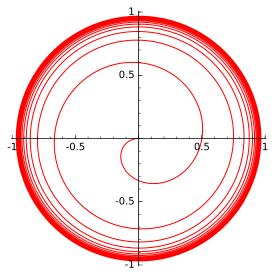
\includegraphics[width=0.5\textwidth]{figs/spiral.pdf}
%  \caption{Polar graph of $r=1- \pi/\theta$}
%\end{figure}
%            \begin{figure}
%  \centering
%    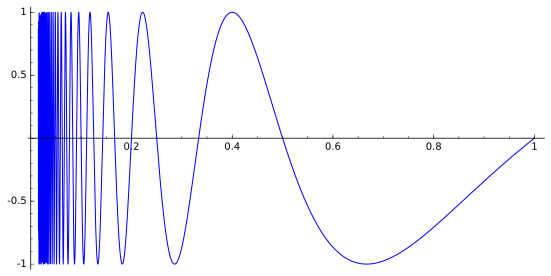
\includegraphics[width=0.5\textwidth]{figs/topol.pdf}
%                \caption{Graph of $y = \sin(\pi/x)$}
%\end{figure}
        \item First we show that the maps $f(\theta) = (1-\pi/\theta, \theta)$ and $g(x) = (x,\sin(\pi/x)$ where $\theta\geq \pi$ and $0<x\leq 1$ are both homeomorphisms by proving they are continuous, injective and their inverse is continuous. 
            
            For both cases, $f$ and $g$ are continuous because each of its component functions are continuous (on its respective domains). Also, both functions are injective because  the second component of $f(\theta) $ and the first one of $g(x)$ are just the identity. The inverse of $f$ and $g$ are just the second and first projection respectively, therefore they are both continuous. 

            Since the sets (we proved this in the last homework) $[\pi,\infty)$ and $(0,1]$ are homeomorphic, namely $h(\theta)=x$, we conclude that $\X$ and $\Y$ are homeomorphic with the homeomorphism $p\mapsto (g\circ h\circ f^{-1 })(p)$ for all $p\in \X$.

\item Both $\X$ and $\Y$ are the image of connected spaces over continuous functions and therefore connected. In general, the closure of a connected set is connected because points in the closure cannot be separated from the original. So it is not possible to find a neighborhood of a point in $\bar\X \backslash \X$ of $\bar\Y \backslash \Y$ that is disjoint from $\X$ and $\Y$ respectively. This implies that $\bar\X$ and $\bar\Y$ are connected.

    Next we show that $\Y$ is not path connected. Assuming it is, take a continuous function $\gamma\ :\ [0,1]\to \Y$ such that $\gamma(0) = (0,0)$ and $\gamma(1) = (1, 0)$. Let us assume that if $\gamma_1(t)$ is the first component of the $\gamma(t)$ vector, then $\gamma_1(t)>0$ whenever $t>0$. 
        
        Note that $\gamma$ can always be taken this way since it is continous and this implies that the set $\gamma^{-1 }(\{0 \}\times [-1, 1])$ is closed. It is also bounded since the whole set $\X$ is bounded and therefore it is compact. A compact set in $\R$ always has a largest element which we call $\ell$. Then $\gamma:\ [\ell, 1]$ has the desired property and we can reparametrize.

        The contradiction arises when we take a sequences of values $\{t_n  \}$ converging to zero, then the continuity of $\gamma$ implies that $\gamma(t_n)$ has to converge. Nevertheless, by the intermediate value property applied to the first component $\gamma_1$ we can find a sequence  such that:
        $$\gamma_1(\tau_n)=\frac{\pi}{\frac \pi2 + \pi n} \to 0$$
        For $n\geq 1$ because $\gamma_1$ takes the interval $(0,1)$ to $(0,1)$ by construction. But this means that:
        $$\gamma(\tau_n)=\left(\frac{\pi}{\frac \pi2 + \pi n} , \sin(\frac \pi2 + \pi n) \right) = \left(\frac{\pi}{\frac \pi2 + \pi n} , (-1)^n \right)$$

        Which does not converge. 

\item Prove that the spaces $\overline{\mathbb{X}}$ and $\overline{\mathbb{Y}}$ are not homeomorphic.
\end{itemize}

\end{soln}
\vspace{1in}


\begin{prob}[3]
The unit three-sphere $\mathbb{S}^3$, center the origin is the subset of $\mathbb{R}^4$, with Cartesian co-ordinates $(t, x, y, z) \in \mathbb{R}^4$ given by the equation $t^2 + x^2 + y^2 + z^2 = 1$.  \\Prove that $\mathbb{S}^3$ is connected.  Is $\mathbb{S}^3$ path connected?  Discuss.
\end{prob}
\begin{soln}
    We will show that the set is path connected, this means it is connected. 

    It is well known that we can write any point  $p\in \S^2$ with spherical coordinates like so:
    \begin{align*}
        x&= \cos(\theta)\sin(\phi)\\
        y&=\sin(\theta)\sin(\phi)\\
        z&= \cos(\phi)
    \end{align*}
    Where $\theta\in [0,2\pi)$ and $\phi\in [0,\pi)$. To parametrize $\S^3$ we introduce a new parameter $\psi\in [0,\pi)$ and map  $\psi$ to a scaled copy of $\S^2$ like so:
    \begin{align*}
        x&= \cos(\theta)\sin(\phi)\textcolor{green}{\sin(\psi)}\\
        y&=\sin(\theta)\sin(\phi)\textcolor{green}{\sin(\psi)}\\
        z&= \cos(\phi)\textcolor{green}{\sin(\psi)}\\
        w&= \textcolor{green}{\cos(\psi)}
    \end{align*}
    Any two points $p,p'$  on $\S^3$ can be written in cartesian coordinates, for example $p=(x,y,z,w)$:
    \begin{align*}
        \theta&= \atan(x,y)\\
        \phi &= \acos\left(z/\sqrt{x^2+y^2}\right)\\
        \psi &= \acos\left(w/\sqrt{x^2+y^2+z^2}\right)
    \end{align*}
    The set $[0,2\pi)\times[0,\pi)^2$ is path connected, and this path connects any two points on $\S^3$.  Since the set is path connected, it is also connected.

\end{soln}
\vspace{1in}




\begin{prob}[4]
For $r$ real, let $\mathbb{C}_r$ be the circle, center the point  $(r, 0) \in \mathbb{R}^2$ and radius $r$. \\ Define the Hawaiian earing, $\mathbb{H}$ and the one-sided Hawaiian earing, $\mathbb{H}_+$ by the formulas:
\[ \mathbb{H} =   \bigcup_{n \in (\mathbb{Z} - \{0\})} \mathbb{C}_{\frac{1}{n}}, \hspace{10pt} \mathbb{H}_+ =   \bigcup_{n \in \mathbb{N}} \mathbb{C}_{\frac{1}{n}}. \] 
Sketch $\mathbb{H}$ and $\mathbb{H}_+$.\\
Are these earings connected, or path connected? Explain. \\
Are $\mathbb{H}_+$ and $\mathbb{H}$ homeomorphic? Explain.\\
Also put $\mathbb{J} =  \bigcup_{n \in \mathbb{N}} \mathbb{C}_{n}$.\\
Sketch the set $\mathbb{J}$.\\
Is $\mathbb{J}$ homeomorphic to $\mathbb{H}$? Explain.\\
Also put $\mathbb{K} =  \bigcup_{r \in (\mathbb{R} - \{0\})} \mathbb{C}_{r}$.\\
Is the set $\mathbb{K}$ homeomorphic to $\mathbb{H}$? Explain.


\end{prob}
\begin{soln}
%
%            \begin{figure}
%  \centering
%    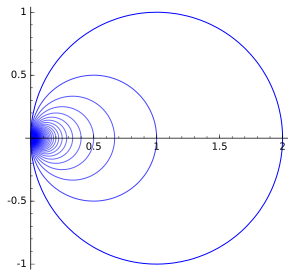
\includegraphics[width=0.5\textwidth]{figs/earing.pdf}
%  \caption{Polar graph of $\HP_+$}
%\end{figure}
%            \begin{figure}
%  \centering
%    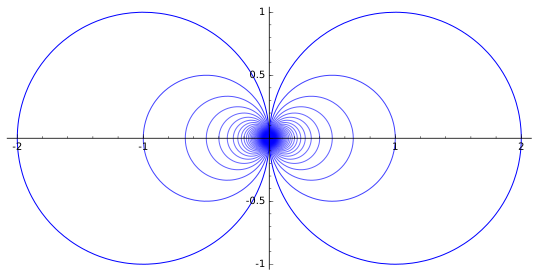
\includegraphics[width=0.5\textwidth]{figs/double.pdf}
%                \caption{Graph of $\HP$}
%\end{figure}

    Both $\HP_+$ and $\HP$ are path connected spaces. These is because all the circles share the origin. More specifically if $x,y\in\HP$ (the proof is identical for $\HP_+$) then these points have to be in some circle say $x\in \C_{1/p}$ and $y\in \C_{1/q}$. Then we can join the path that goes from $x$ to (0,0) through $\C_{1/p} $ with the path that goes from $(0,0)$ to $\C_{1/q}$. Being path connected, the sets are also connected.

    $\HP$ and $\HP_+$ are homeomorphic. An example of a homeomorphism is the map that reflects the circles with even radius across the $y-$axis.

    $\J$ is homeomorphic to $\HP_+$ as it is just the inversion through $\C_1$ (we represent the points as the complex number $z$ for convenience)
    $$I(z) = 1 + \frac 1{\bar z - 1}$$ 
    We showed above that $\HP_+$ and $\HP$ are homeomorphic so we conclude that $\J$ and $\HP$ are also homeomorphic. 

    The sets $\K$ and $H$ are not homeomorphic one reason being that $\K$ contains an open set of $\R^2$ (the whole open circle centered at 1 of radius 1, for example), while $\HP$ does not.
\end{soln}
\vspace{1in}


\begin{prob}[5]
Let $\mathbb{M}$ be the space of all continuous maps $f:[0, 1] \rightarrow \mathbb{R}$, equipped with the distance formula $d(f,g ) =  \sup\{ |f(x) - g(x)|:  x \in [0, 1]\}$.  \\Prove that $d$ gives the space $\mathbb{M}$ a metric.   \\For $n$ a positive integer, let $f_n(x) = x^n$, defined for any $x\in [0, 1]$. \\ Prove that the sequence $\mathbb{F} = \{f_n: n \in \mathbb{N}\}$ has no convergent subsequence. \\ Is $\mathbb{F}$ a Cauchy sequence? Explain. 
\end{prob}
\begin{soln}
First we show it is a metric:
    \begin{enumerate}
        \item For any $f,g\in \M$, we have that $f-g$ is also continuous on $[0,1]$. And, since this is a compact subset of $\R$, $|f-g|$ attains a max value on the interval. This means that $d(f,g)$ exists and is well-defined on all of $\M$. 
        \item Symmetry  and nonnegativeness of $d$ comes from the absolute value since:
            $$|f-g| = |g-f|\geq 0$$
        \item  If $f\neq g$ then there exists $x\in [0,1]$ such that $f(x)-f(x)>0$. Therefore, $d(f,g)>0$. 
        \item For all $x\in [0,1]$ and all $f,g,h\in \M$ we have that:
            $$|f(x) - g(x)| \leq |f(x)-h(x)| + | h(x) - g(x)|$$
            including the value  $x_0$ where $d(f,g)$ is attained. Then we can conclude the triangle inequality by observing:
            $$d(f,g) \leq |f(x_0) - h(x_0)| + | h(x_0) - g(x_0)| \leq d(f,h) + d(h,g)$$

            For any point $0\leq x <1$ we have that when $n\to \infty$, $x^n\to 0$. This implies that any convergent subsequence of $\{ f_n \}$ would have to converge to $f(0)=0$ for all $0\leq x<1$. Also, $f$ needs to be continuous  and this means that $f =0$. On the other hand, for all $n\in \N$ we have that: $f_n(1)=1$ then any subconverging sequence would have to converge to a function $f$ that also satisfies this condition. This gives a contradiction as $f(1)=0$ and $f(1)=1$.

            The sequence $f_n$ is not Cauchy with this metric. To see this we find the max of $x^n-x^m$ in the interval. The critical point are:
            $$nx^{n-1} - mx^{m-1}=0$$
            Assuming that $n>m$ and that $x\neq 0$ we get that:
            $$ x=\left( \frac mn\right)^{\frac 1{n-m}}$$
            Since the function $x^n-x^m$ is continuous and is zero at $x=0,1$ the distance has to be positive at some point $0<x<1$. Substituting this value in the original equation:
            $$\left( \frac mn\right)^{\frac n{n-m}}-\left( \frac mn\right)^{\frac m{n-m}}= \left( \frac mn\right)^{\frac m{n-m}}\left( \frac mn - 1\right)$$
            And taking $n=m^2$ and $m\to \infty $ we get:
            $$\left(\frac 1m \right)^{\frac 1{m-1}}\left(1/m - 1\right)$$
            And this goes to -1 when $m\to \infty$ (with the absolute value it would go to 1).


    \end{enumerate}
\end{soln}
\vspace{1in}


\begin{prob}[6]
Prove that the closed real interval $[0, 1]$ cannot be written as a countably infinite disjoint union of intervals, each open in $[0, 1]$. 
\end{prob}
\begin{soln}

\end{soln}
\vspace{1in}



\end{document}








